\documentclass[11pt]{article} 
\usepackage[english]{babel}
\usepackage[utf8]{inputenc}
\usepackage[margin=0.5in]{geometry}
\usepackage{amsmath}
\usepackage{amsthm}
\usepackage{amsfonts}
\usepackage{amssymb}
\usepackage[usenames,dvipsnames]{xcolor}
\usepackage{graphicx}
\usepackage[siunitx]{circuitikz}
\usepackage{tikz}
\usepackage[colorinlistoftodos, color=orange!50]{todonotes}
\usepackage{hyperref}
\usepackage[numbers, square]{natbib}
\usepackage{fancybox}
\usepackage{epsfig}
\usepackage{soul}
\usepackage[framemethod=tikz]{mdframed}
\usetikzlibrary{positioning, automata, backgrounds}
\usepackage[shortlabels]{enumitem}
\usepackage[version=4]{mhchem}
\usepackage{multicol}
\usepackage{forest}
\usepackage{mathtools}
\usepackage{comment}
\usepackage{enumitem}
\usepackage[utf8]{inputenc}
\usepackage[linesnumbered,ruled,vlined]{algorithm2e}
\usepackage{listings}
\usepackage{color}
\usepackage[numbers]{natbib}
\usepackage{subfiles}
\usepackage{tkz-berge}


\newtheorem{prop}{Proposition}[section]
\newtheorem{thm}{Theorem}[section]
\newtheorem{lemma}{Lemma}[section]
\newtheorem{cor}{Corollary}[prop]

\theoremstyle{definition}
\newtheorem{definition}{Definition}

\theoremstyle{definition}
\newtheorem{required}{Problem}

\theoremstyle{definition}
\newtheorem{ex}{Example}

\newcommand{\interval}[4]{\draw (#2, #1) -- (#3, #1); % Usage: \interval{height}{start}{end}{label}
\draw (#2, #1-0.11) -- (#2, #1+0.11); % draw left whisker
\draw (#3, #1-0.11) -- (#3, #1+0.11); % draw right whisker
\node[] at (#2-0.25, #1) {#4};
}


\setlength{\marginparwidth}{3.4cm}
%#########################################################

%To use symbols for footnotes
\renewcommand*{\thefootnote}{\fnsymbol{footnote}}
%To change footnotes back to numbers uncomment the following line
%\renewcommand*{\thefootnote}{\arabic{footnote}}

% Enable this command to adjust line spacing for inline math equations.
% \everymath{\displaystyle}

% _______ _____ _______ _      ______ 
%|__   __|_   _|__   __| |    |  ____|
%   | |    | |    | |  | |    | |__   
%   | |    | |    | |  | |    |  __|  
%   | |   _| |_   | |  | |____| |____ 
%   |_|  |_____|  |_|  |______|______|
%%%%%%%%%%%%%%%%%%%%%%%%%%%%%%%%%%%%%%%

\title{
\normalfont \normalsize 
\textsc{CSCI 3104 Spring 2022 \\ 
Instructors: Profs. Chen and Layer} \\
[10pt] 
\rule{\linewidth}{0.5pt} \\[6pt] 
\huge Problem Set 1 \\
\rule{\linewidth}{2pt}  \\[10pt]
}
%\author{}
\date{}

\begin{document}

\definecolor {processblue}{cmyk}{0.96,0,0,0}
\definecolor{processred}{rgb}{200, 0, 0}
\definecolor{processgreen}{rgb}{0, 255, 0}
\DeclareGraphicsExtensions{.png}
\DeclareGraphicsExtensions{.gif}
\DeclareGraphicsExtensions{.jpg}

\maketitle


%%%%%%%%%%%%%%%%%%%%%%%%%
%%%%%%%%%%%%%%%%%%%%%%%%%%
%%%%%%%%%%FILL IN YOUR NAME%%%%%%%
%%%%%%%%%%AND STUDENT ID%%%%%%%%
%%%%%%%%%%%%%%%%%%%%%%%%%%
\noindent
Due Date \dotfill January 25, 2022 \\
Name \dotfill \textbf{Your Name} \\
Student ID \dotfill \textbf{Your Student ID} \\
Collaborators \dotfill \textbf{List Your Collaborators Here}

\tableofcontents

\section{Instructions}
 \begin{itemize}
	\item The solutions \textbf{should be typed}, using proper mathematical notation. We cannot accept hand-written solutions. \href{http://ece.uprm.edu/~caceros/latex/introduction.pdf}{Here's a short intro to \LaTeX.}
	\item You should submit your work through the \textbf{class Canvas page} only. Please submit one PDF file, compiled using this \LaTeX \ template.
	\item You may not need a full page for your solutions; pagebreaks are there to help Gradescope automatically find where each problem is. Even if you do not attempt every problem, please submit this document with no fewer pages than the blank template (or Gradescope has issues with it).

	\item You are welcome and encouraged to collaborate with your classmates, as well as consult outside resources. You must \textbf{cite your sources in this document.} \textbf{Copying from any source is an Honor Code violation. Furthermore, all submissions must be in your own words and reflect your understanding of the material.} If there is any confusion about this policy, it is your responsibility to clarify before the due date. 

	\item Posting to \textbf{any} service including, but not limited to Chegg, Reddit, StackExchange, etc., for help on an assignment is a violation of the Honor Code.

	\item You \textbf{must} virtually sign the Honor Code (see Section \ref{HonorCode}). Failure to do so will result in your assignment not being graded.
\end{itemize}


\section{Honor Code (Make Sure to Virtually Sign)} \label{HonorCode}

\begin{required}
\begin{itemize}
\item My submission is in my own words and reflects my understanding of the material.
\item Any collaborations and external sources have been clearly cited in this document.
\item I have not posted to external services including, but not limited to Chegg, Reddit, StackExchange, etc.
\item I have neither copied nor provided others solutions they can copy.
\end{itemize}

%\noindent In the specified region below, clearly indicate that you have upheld the Honor Code. Then type your name. 
\end{required}

\begin{proof}[Agreed (signature here).]
%% Typing "I agree to the above," followed by your name is sufficient.
\end{proof}


\newpage
\section{Standard 1- Proof by Induction}

\subsection{Problem \ref{Induction1}}
\begin{required} \label{Induction1}
A student is trying to prove by induction that $3^{n} < n!$ for $n \geq 7$. 

\begin{proof}[Student's Proof]
The proof is by induction on $n \geq 7$. 
\begin{itemize}
\item \textbf{Base Case:} When $n = 7$, we have that:
\begin{align*}
3^{7} &= 2187 \\
&< 5040 \\
&= 7!
\end{align*}

\item \textbf{Inductive Hypothesis:} Now suppose that for all $k \geq 7$ we have that $3^{k} < k!$. 

\item \textbf{Inductive Step:} We now consider the $k+1$ case. We have that $3^{k+1} < (k+1)!$. It follows that $3^{k} < k!$. The result follows by induction.
\end{itemize}
\end{proof}

There are two errors in this proof. 
\begin{enumerate}[label=(\alph*)]
\item The Inductive Hypothesis is not correct. Write an explanation to the student explaining why their Inductive Hypothesis is not correct.  [\textbf{Note:} You are being asked to explain why the Inductive Hypothesis is wrong, and \textbf{not} to rewrite a corrected Inductive Hypothesis.]


\begin{proof}[Answer]
%Your answer goes here
\end{proof}



\vskip 15pt
\item The Inductive Step is not correct. Write an explanation to the student explaining why their Inductive Step is not correct. [\textbf{Note:} You are being asked to explain why the Inductive Step is wrong, and \textbf{not} to rewrite a corrected Inductive Step.]

\begin{proof}[Answer]
%Your answer goes here
\end{proof}
\end{enumerate}
\end{required}





\newpage
\subsection{Problem \ref{Induction2}} 
\begin{required} \label{Induction2}
Consider the sequence $T_n,~n\geq 1$ defined by the following recurrence: $T_1=T_2=T_3=1$ and $T_n=T_{n-1}+T_{n-2}+T_{n-3}$ for $n\geq 4$. \\

\noindent Prove by induction that $T_{n} < 2^n$ for all $n\geq 1$. 
\end{required}

\begin{proof}
%Your proof goes here.
\end{proof}



\newpage
\subsection{Problem \ref{Induction3}}
\begin{required} \label{Induction3}
The complete, balanced ternary tree of depth $d$, denoted $\mathcal{T}(d)$, is defined as follows. 
\begin{itemize}
\item $\mathcal{T}(0)$ consists of a single vertex.
\item For $d > 0$, $\mathcal{T}(d)$ is obtained by starting with a single vertex and setting each of its three children to be copies of $\mathcal{T}(d-1)$.
\end{itemize}

\noindent Prove by induction that $\mathcal{T}(d)$ has $3^{d}$ leaf nodes. To help clarify the definition of $\mathcal{T}(d)$, illustrations of $\mathcal{T}(0), \mathcal{T}(1)$, and $\mathcal{T}(2)$ are on the next page. [\textbf{Note:} $\mathcal{T}(d)$ is a tree and \textbf{not} the number of leaves on the tree. Avoid writing $\mathcal{T}(d) = 3^{d}$, as these data types are incomparable: a tree is not a number.]
\end{required}

\begin{proof}
%Your proof goes here
\end{proof}

\newpage
\begin{ex}
We have the following:

\begin{center}
\begin{forest}
    for tree={
        circle,
        draw,
        fill,
        minimum width=2pt, % size
        inner sep=0pt,
        parent anchor=center,
        child anchor=center,
        s sep+=25pt, % distance between children
    }
[  ]
\end{forest}
\noindent \\ $\mathcal{T}(0)$.
\end{center}

\begin{center}
\begin{forest}
    for tree={
        circle,
        draw,
        fill,
        minimum width=2pt, % size
        inner sep=0pt,
        parent anchor=center,
        child anchor=center,
        s sep+=25pt, % distance between children
    }
[ [] [] [] ]
\end{forest}
\noindent \\ $\mathcal{T}(1)$.
\end{center}


\begin{center}
\begin{forest}
    for tree={
        circle,
        draw,
        fill,
        minimum width=2pt, % size
        inner sep=0pt,
        parent anchor=center,
        child anchor=center,
        s sep+=25pt, % distance between children
    }
[ [[] [][] ] [[] [][] ] [[] [][] ] ]
\end{forest}
\noindent \\ $\mathcal{T}(2)$.
\end{center}
\end{ex}

%%%%%%%%%%%%%%%%%%%%%%%%%%%%%%%%%%%%%%%%%%%%%%%%%%


\newpage
\section{Standard 2- Examples Where Greedy Algorithms Fail}

\subsection{Problem \ref{GreedyFail1}}
\begin{required} \label{GreedyFail1}
Recall the \textsf{Interval Scheduling} problem, where we take as input a set of intervals $\mathcal{I}$. The goal is to find a maximum-sized set $S \subseteq \mathcal{I}$, where no two intervals in $S$ intersect. Consider the greedy algorithm where we place all of the intervals of $\mathcal{I}$ into a priority queue, ordered earliest start time to latest start time. We then construct a set $S$ by adding intervals to $S$ as we poll them from the priority queue, provided the element we polled does not intersect with any interval already in $S$. \\

\noindent Provide an example with at least $5$ intervals where this algorithm fails to yield a maximum-sized set of pairwise non-overlapping intervals. Clearly specify both the set $S$ that the algorithm constructs, as well a larger set of pairwise non-overlapping intervals. \\

\noindent You may explicitly specify the intervals by their start and end times (such as in the examples from class) or by drawing them. \textbf{If you draw them, please make it very clear whether two intervals overlap.} You are welcome to hand-draw and embed an image, provided it is legible and we do not have to rotate our screens to grade your work. Your justification should still be typed. If you would prefer to draw the intervals using \LaTeX, we have provided sample code below.
\end{required}


%Sample code to draw intervals
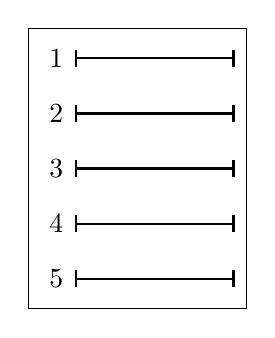
\begin{tikzpicture}[thick, framed]   
\interval{3.3}{5}{7}{1}
\interval{2.6}{5}{7}{2}
\interval{1.9}{5}{7}{3}
\interval{1.2}{5}{7}{4}
\interval{0.5}{5}{7}{5}
\end{tikzpicture}

\begin{proof}[Answer]
%Your answer here.
\end{proof}






\newpage
\subsection{Problem \ref{GreedyFail3}}
\begin{required} \label{GreedyFail3}
Consider now the \textsf{Weighted Interval Scheduling} problem, where each interval $i$ is specified by 
\[
([\text{start}_{i}, \text{end}_{i}], \text{weight}_{i}). 
\]

\noindent Here, the weight is an assigned value that is independent of the length $\text{end}_{i} - \text{start}_{i}$. Here, you may assume $\text{weight}_{i} > 0$. We seek a set $S$ of pairwise non-overlapping intervals that maximizes $\sum_{i \in S} \text{weight}_{i}$. That is, rather than maximizing the number of intervals, we are seeking to maximize the sum of the weights. \\

\noindent Consider a greedy algorithm which works identically as in Problem \ref{GreedyFail1}. Draw an example with at least 5 appointments where this algorithm fails. Show the order in which the algorithm selects the intervals, and also show a subset with larger weight of non-overlapping intervals than the subset output by the greedy algorithm. The same comments apply here as for Problem \ref{GreedyFail1} in terms of level of explanation.
\end{required}

\begin{proof}[Answer]
%Your answer here.
\end{proof}




\newpage
\section{Standard 3- Exchange Arguments}
\subsection{Problem \ref{Exchange1}}
\begin{required} \label{Exchange1}
Recall the Making Change problem, where we have an infinite supply of pennies (worth $1$ cent), nickels (worth $5$ cents), dimes (worth $10$ cents), and quarters (worth $25$ cents). We take as input an integer $n \geq 0$. The goal is to make change for $n$ using the fewest number of coins possible. \\

\noindent Prove that in an optimal solution, we use at most $2$ dimes. 
\end{required}

\begin{proof}
%Your proof here
\end{proof}



\newpage
\subsection{Problem \ref{Exchange2}}

\begin{required} \label{Exchange2}
Consider the \textsf{Interval Projection} problem, which is defined as follows.
\begin{itemize}
\item \textsf{Instance:} Let $\mathcal{I}$ be a set of intervals on the real line.
\item \textsf{Solution:} A minimum sized set $S$ of points on the real line, such that (i) for every interval $[s, f] \in \mathcal{I}$, there exists a point $x \in S$ where $x$ is in the interval $[s, f]$. We call $S$ a \textit{projection set}.
\end{itemize}

\noindent Do the following.
\begin{enumerate}[label=(\alph*)]
\subsubsection{Problem 7\ref{6a}}
\item \label{6a} Find a minimum sized projection set $S$ for the following set of intervals:
\begin{align*}
\mathcal{I} = \{ [0, 1], [0.5, 1], [0.9, 1.5], [1.2, 2], [1.7, 2.3] \}.
\end{align*}


\begin{proof}[Answer]
%Your Answer Here
\end{proof}

\newpage
\subsubsection{Problem 7\ref{6b}}
\item \label{6b} Fix a set of intervals $\mathcal{I}$, and let $S$ be a projection set. Prove that there exists a projection set $S^{\prime}$ such that (i) $|S^{\prime}| = |S|$, and (ii) where every point $x \in S^{\prime}$ is the right end-point of some interval $[s, f] \in \mathcal{I}$. 

\begin{proof}
%Your proof here
\end{proof}

\end{enumerate}
\end{required}

\newpage
\section{Standard 4- Huffman coding}
\subsection{Problem \ref{Huffman}}
\begin{required} \label{Huffman}
Given an alphabet of five symbols: a, b, c, d and e, with frequencies 0.4, 0.12, 0.2, 0.15, and 0.13
respectively, work out the Huffman codes for the symbols. You need to first show the optimal binary tree you construct, and then write down the corresponding codes. \\
\end{required}



\begin{proof}[Answer]
%Your answer here
\end{proof}



%%%%%%%%%%%%%%%%%%%%%%%%%%%%%%%%%%%%%%%%%%%%%%%%%%

\end{document} % NOTHING AFTER THIS LINE IS PART OF THE DOCUMENT



